\documentclass{article}

\usepackage[margin=1in]{geometry} 
\usepackage{amsmath,amsthm,amssymb}
\usepackage[utf8]{inputenc} 
\usepackage{color}
\usepackage{tikz}
\usepackage{cancel}
\usepackage[linewidth=1pt]{mdframed}
\usepackage{pgfplots}

\usetikzlibrary{positioning}

\newcommand{\R}{\mathbb{R}}  
\newcommand{\Z}{\mathbb{Z}}
\newcommand{\N}{\mathbb{N}}
\newcommand{\Q}{\mathbb{Q}}
\newcommand{\C}{\mathbb{C}}

\newcommand{\argmin}{\operatornamewithlimits{argmin }}
\newcommand{\argmax}{\operatornamewithlimits{argmax }}

\newenvironment{theorem}[2][Theorem]{\begin{trivlist}
\item[\hskip \labelsep {\bfseries #1}\hskip \labelsep {\bfseries #2.}]}{\end{trivlist}}
\newenvironment{lemma}[2][Lemma]{\begin{trivlist}
\item[\hskip \labelsep {\bfseries #1}\hskip \labelsep {\bfseries #2.}]}{\end{trivlist}}
\newenvironment{exercise}[2][Exercise]{\begin{trivlist}
\item[\hskip \labelsep {\bfseries #1}\hskip \labelsep {\bfseries #2.}]}{\end{trivlist}}
\newenvironment{problem}[2][Problem]{\begin{trivlist}
\item[\hskip \labelsep {\bfseries #1}\hskip \labelsep {\bfseries #2.}]}{\end{trivlist}}
\newenvironment{question}[2][Question]{\begin{trivlist}
\item[\hskip \labelsep {\bfseries #1}\hskip \labelsep {\bfseries #2.}]}{\end{trivlist}}
\newenvironment{corollary}[2][Corollary]{\begin{trivlist}
\item[\hskip \labelsep {\bfseries #1}\hskip \labelsep {\bfseries #2.}]}{\end{trivlist}}

\newenvironment{solution}{\begin{proof}[Solution]}{\end{proof}}

\newlength\tindent
\setlength{\tindent}{\parindent}
\setlength{\parindent}{0pt}
\renewcommand{\indent}{\hspace*{\tindent}}

\def\cunderline#1#2{\color{#1}\underline{{\color{black}#2}}\color{black}}
\def\cunderbrace#1#2{\color{#1}\underbrace{{\color{black}#2}}\color{black}}

\newcommand{\tikzmark}[1]{\tikz[baseline,remember picture] \coordinate (#1) {};}

\usepackage{hyperref}

\usetikzlibrary{patterns}

\newcommand{\Napp}{\mathcal{N}}
\newcommand{\Dapp}{\mathcal{D}}
\newcommand{\Oapp}{\mathcal{O}}
\newcommand{\Lapp}{\mathcal{L}}

\begin{document}


\title{Modèles de melange (G.M.M) \\ Cours 2}
\author{} 
\date{}

\maketitle

\section{Introduction}

\subsection{Clustering:}
Apprentissage non-supervisé\\
$\Dapp = (\underbrace{\vec{x_n}}_{\R^d})^N_{n=1}$, on fix $K$, un nombre de clusters
\vspace{1em}

\underline{ex:} K-means\\
Algo iteratif:
\vspace{1em}

\hspace*{9px} 0) Choisir une distance *\\
$\left[
\begin{array}{l}
\text{1) Assignation}\\
\text{\indent pour chaque cluster: }\vec{m_k}\text{, }\vec{x_n} \in\text{ au cluster le plus proche (min distance }(\vec{x_n},\vec{m_k}))\\
\text{2) Re-estimation}\\
\text{\indent recalculer les }(\vec{m_k})^K_{k=1}
\end{array}
\right.$

\subsection{Estimation de distribution:}

ex: classification (d'image)\\

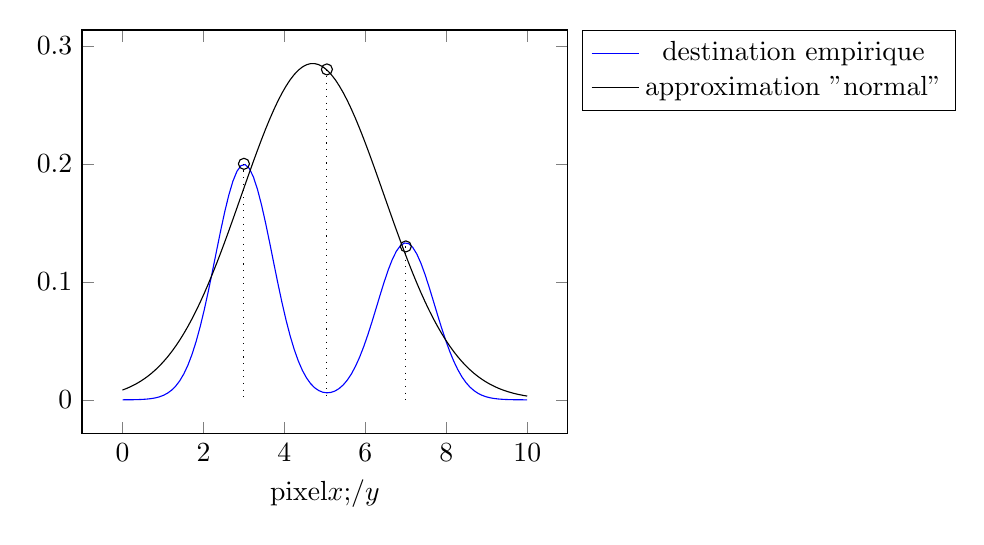
\begin{tikzpicture}
\begin{axis}[scale=0.9, scaled y ticks = false, xlabel=$\text{pixel} x\text{;}/y$, legend pos=outer north east]
\addplot[domain=0:10, samples=100, color=blue]{1/(1*sqrt(6.282))*exp(-(x-3)^2/(1^2))/2 + 1/(1*sqrt(6.282))*exp(-(x-7)^2/(1^2))/3}; 
\addlegendentry{destination empirique}
\draw[dotted] (axis cs:3,0.2) -- (axis cs:3,0);
\draw (axis cs:3,0.2) circle (2pt);
\draw[dotted] (axis cs:7,0.13) -- (axis cs:7,0);
\draw (axis cs:7,0.13) circle (2pt);
\addplot[domain=0:10, samples=100, color=black]{5/(1*sqrt(6.282))*exp(-((x-4.7)*2)^2/(5^2))/7}; 
\addlegendentry{approximation "normal"}
\draw[dotted] (axis cs:5.05,0.28) -- (axis cs:5.05,0);
\draw (axis cs:5.05,0.28) circle (2pt);
\end{axis}
\end{tikzpicture}
\\

$\rightarrow$ augmenter la capacité du modèle\\
$\rightarrow$ augmenter le nombre de paramètres\\

\subsection{Mélange de Gaussienne (GMM):}
$K$ le nombre de Gaussienne / cluster\\
$$p(\vec{x_n}|\underbrace{\Oapp}_{(\Pi_k,\vec{\mu_k},\Sigma_k)^K_{k=1}}) = \sum^K_{k=1}\underbrace{\Pi_k}_{\text{Poids du mélange}} \underbrace{\Napp(\vec{\mu_k}, \Sigma_k)}_{\text{la gaussienne}}$$\\

\underline{Estimer les paramètres du mélange}
\vspace{1em}

$\rightarrow$ maximiser $\prod^N_{n=1} P(\vec{X}=\vec{x_n}|\Oapp)$\\
$\rightarrow$ maximiser $\log( \prod^N_{n=1} \underbrace{P(\vec{X}=\vec{x_n}|\Oapp)}_{\sum^K_{k=1}\Pi_k\Napp(\vec{\mu_k}, \Sigma_k)})$\\

\section{Algorithme E.M}
\textbullet Algo iteratif qui cherche à maximiser $$\log(P(\vec{X}=\vec{x_n}|\Oapp))$$\\
\textbullet Introduire des variable \underline{latentes} (cachéés): $$\text{pour chaque } \vec{x} \rightarrow \vec{Z}$$\\
$$\vec{Z} = \left( \begin{array}{l} 0\\0\\1\tikzmark{Zks}\\0\\0 \end{array} \right)\ \ \tikzmark{Zke}\vec{Z_k} = 1 \Leftrightarrow \vec{x}\in\text{ cluster k}$$\\
\begin{tikzpicture}[overlay,remember picture]
	\node (Zke2) [above left=0em and 0em of Zke]{};
    \draw[-<, in=0, out=180] (Zks.east)++(0.3em,0.4em) to (Zke2.west);
\end{tikzpicture}

$\vec{Z}:$ \textbullet pseudo affectation\\
\indent \textbullet une vecteur latent\\
\indent \textbullet inconnue $\Rightarrow \vec{Z}$ un vecteur aléatoire\\
\indent \textbullet affectation "soft": un point peut appartenire à tous les clusters.\\
\vspace{1em}

\underline{Résumé des programes}\\
Introduction $\vec{Z}$ associé à $\vec{X}$\\
Si on souhaite maximiser\\
$$P(\vec{X}|\underline{\underline{\Oapp}}) = \sum_Z P(\vec{X},\vec{Z}|\Oapp)$$
$$P(\vec{X}|\Oapp) = \underbrace{\sum_Z P(\vec{X}|\vec{Z},\Oapp)}_{\Napp(\vec{\mu_k},\Sigma_k)} \underbrace{P(\vec{Z}|\Oapp)}_{\Pi_k}$$
\vspace{1em}

si $\vec{Z_k} = \left( \begin{array}{l} 0\\0\\1\tikzmark{Zk2s}\\0\\0 \end{array} \right)\ \ \tikzmark{Zk2e}k$\\ 
\begin{tikzpicture}[overlay,remember picture]
	\node (Zk2e2) [above left=0em and 0em of Zk2e]{};
    \draw[-<, in=0, out=180] (Zk2s.east)++(0.3em,0.4em) to (Zk2e2.west);
\end{tikzpicture}
\textbullet $(\vec{X},\vec{Z})$: données complètes\\
\textbullet $(\vec{X})$: données incomplètes
\vspace{1em}

\underline{étape E(xpection):}\\
\indent $\rightarrow$ connaître $\vec{Z}$ \color{red}\underline{\underline{à $\Oapp$ fixé}} \color{black}\\
\indent $\rightarrow$ calcul la probabilité d'affectation: $P(\vec{Z}|\vec{X},\Oapp)$
\vspace{1em}

\underline{étape M(aximigation)}\\
\indent Les données sont complètes\\
\indent $\Rightarrow$ calcule de $\Oapp$ \color{red}, on "fixe" $\vec{Z}$ \color{black}

\section{Optimisation variationelle}
On souhaite maxmiser selon $\Oapp:$\\
$$\log(P(\vec{X}|\Oapp) = \sum_{\vec{Z}} q(\vec{Z})\log\frac{P(\vec{X},\vec{Z}|\Oapp)}{q(\vec{Z})} - \sum_{\vec{Z}} q(\vec{Z})\log\frac{P(\vec{X}|\vec{Z},\Oapp)}{q(\vec{Z})}$$
\vspace{1em}

\textbullet Après l'introduction de $\vec{Z}$, on introduit un distribution auxiliaire sur $\vec{Z}$: $q(\vec{Z})$
\vspace{1em}

\underline{rappel:} 
$$P(\vec{X}|O) = \frac{P(\vec{X},\vec{Z}|\Oapp)}{P(\vec{X}|\vec{Z},\Oapp)}$$
$$\Rightarrow \log P(\vec{X}|\Oapp) = \log(P(\vec{X},\vec{Z}|\Oapp) - \log(P(\vec{X}|\vec{Z},\Oapp)$$\\

\underline{c.à.d:}\\
\indent le 2eme terme
$$-\sum_{\vec{Z}}q(\vec{Z})\log\left( \frac{P(\vec{Z}|\vec{X},\Oapp)}{q(\vec{Z})} \right) = E_{\vec{Z}~q(\vec{Z})} \left[ \log \frac{P(\vec{Z},\vec{X}|\Oapp)}{q(\vec{Z})} \right]$$
\underline{\underline{Divergence}} de Kullback-leiber ($D_{KL}$)\\
$$D_{KL}(\tikzmark{q}q(\vec{Z})||\tikzmark{P}P(\vec{Z}|\vec{X},\Oapp))$$
\begin{tikzpicture}[overlay,remember picture]
    \node (Dd) [below right of = P, node distance = 4 em, anchor=west]{\footnotesize \text{deux distribution sur $\vec{Z}$}};
    \draw[<-, in=180, out=-90] (q.south)++(0.5em,-1em) to (Dd.west);
    \draw[<-, in=180, out=-90] (P.south)++(2.5em,-1em) to (Dd.west);

\end{tikzpicture}
\vspace{1em}

Divergence $\neq$ distance (asymétrique)\\
%\textbullet Ssi q=P FIXME :(

\underline{\textbullet 1er terme:}\\
$$E_{\vec{Z}~q(\vec{Z})} \left[ \log \frac{P(\vec{Z},\vec{X}|\Oapp)}{q(\vec{Z})} \right]$$
$\rightarrow$ ELBO (Evidence Lower Bound)\\
$$\log(P(\vec{X}|\Oapp)) = \underbrace{\Lapp(\Oapp,q)}_{\text{ELBO } \geq\underbrace{\Lapp(\Oapp,q)}_{\text{borne inf}}} + D_{KL}(q(\vec{Z})||P(\vec{Z}|\vec{X},\Oapp))$$

\subsection{Etape E}
\textbullet Les paramètres sont fixés: $\Oapp = \Oapp^{\text{ old}}$\\
\textbullet Maximiser $\Lapp(\Oapp^{\text{ old}},q)$
$$\rightarrow \Lapp(\Oapp^{\text{ old}},q) = - D_{KL}(q(\vec{Z})||P(\vec{Z}|\vec{X},\Oapp^{\text{ old}})) + \underbrace{\color{red}\bcancel{\color{black}\log(P(\vec{X}|\Oapp^{\text{ old}}))}}_{\color{red}cte}$$
$$\Rightarrow q(\vec{Z})=P(\vec{Z}|\vec{X},\Oapp^{\text{ old}})$$

\subsection{Etape M}
Maximiser $\Lapp$ selon $\Oapp$ avec $q$ fixé
\vspace{1em}

\underline{Illustration:} 
\vspace{2em}

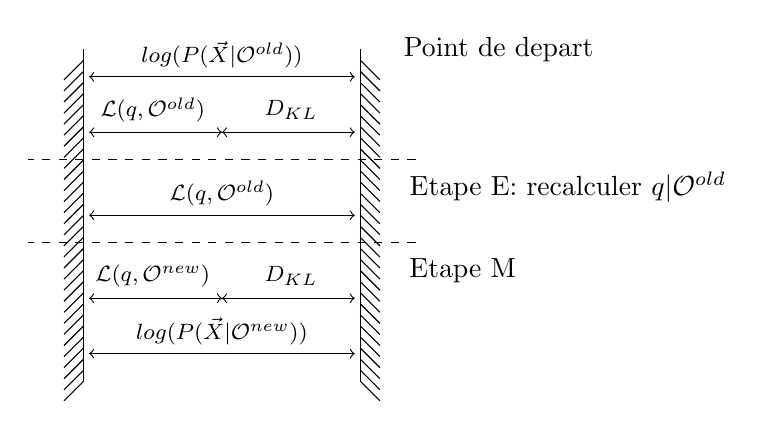
\begin{tikzpicture}

\tikzstyle{left}=[postaction={draw,decorate,decoration={border,angle=135, amplitude=1em,segment length=0.4em}}]
\tikzstyle{right}=[postaction={draw,decorate,decoration={border,angle=-135, amplitude=1em,segment length=0.4em}}]
\draw[left] (0em,-2em) to (0em, 10em);
\draw[right] (10em,-2em) to (10em, 10em);

\node at (15em, 10em)   (Pdd) {\text{Point de depart}};

\node at (5em, 9.8em)   (logOld) {\footnotesize $log(P(\vec{X}|\Oapp^{old}))$};
\draw[<->] (9.8em,9em) to (0.2em, 9em);

\node at (2.5em, 7.8em)   (LOld1) {\footnotesize $\Lapp(q,\Oapp^{old})$};
\node at (7.5em, 7.8em)   (DKLOld) {\footnotesize $D_{KL}$};
\draw[<->] (9.8em,7em) to (5em, 7em);
\draw[<->] (5em,7em) to (0.2em, 7em);

\draw[dashed] (12em,6em) to (-2em, 6em);
\node at (17.5em, 5em)   (EE) {\text{Etape E: recalculer $q|\Oapp^{old}$}};

\node at (5em, 4.8em)   (LOld2) {\footnotesize $\Lapp(q,\Oapp^{old})$};
\draw[<->] (9.8em,4em) to (0.2em, 4em);

\draw[dashed] (12em,3em) to (-2em, 3em);
\node at (13.7em, 2em)   (EM) {\text{Etape M}};

\node at (2.5em, 1.8em)   (LNew1) {\footnotesize $\Lapp(q,\Oapp^{new})$};
\node at (7.5em, 1.8em)   (DKLNew) {\footnotesize $D_{KL}$};
\draw[<->] (9.8em,1em) to (5em, 1em);
\draw[<->] (5em,1em) to (0.2em, 1em);

\node at (5em, -0.2em)   (logNew) {\footnotesize $log(P(\vec{X}|\Oapp^{new}))$};
\draw[<->] (9.8em,-1em) to (0.2em, -1em);


\end{tikzpicture}

\vspace{5em}

\url{https://en.wikipedia.org/wiki/Expectation%E2%80%93maximization_algorithm}
\end{document}
